\section{Tekniske Overvejelser}
Something something

\subsection{Programstruktur}
Vi valgte helt fra starten at bygge vores program op omkring MVVM(Model-View-ViewModel) mønstret, som er en variation af Martin Fowler's Presentation Model (KILDE https://martinfowler.com/eaaDev/PresentationModel.html). Vi valgte MVVM, da det spiller godt sammen med JavaFX.

\begin{figure}[h!]
	\centerline{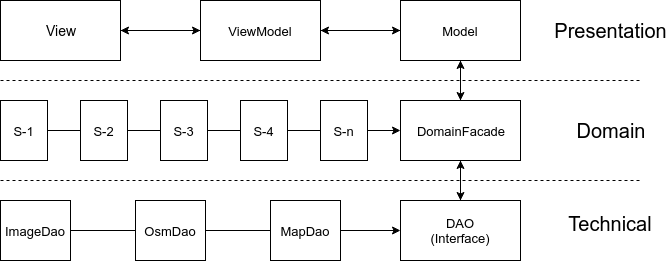
\includegraphics[width=13 cm]{Figurer/structure.png}}
	\caption{Test}
	\label{fig:structure}
\end{figure}

\subsection{Binært Format}
Mappr's binære format benytter Java's inbyggede objekt serialisering.(KILDE https://docs.oracle.com/javase/9/docs/specs/serialization/index.html)
Som datagrundlag for vores serialiserede fil, bruger vi vores MapData klasse som ses på Figur \ref{fig:mapdata}. Indholdet af MapData klassen var op til debat flere gange under projektforløbet, men vi endte med kun at gemme Points of Interest - udover resultatet af vores OSM parsing.
En anden mulighed ville have været også at gemme KD-Træet og Dijkstra grafen på disken, hvilket muligvis ville have formindsket time-to-load, men da Danmark i forvejen fyldte lidt over 500MB på disken, valgte vi at lave det tradeoff.

\begin{figure}[h!]
    \begin{lstlisting}
	@Data
	@Builder
	public class MapData implements Serializable {
		private Boundaries boundaries;
		private Vector<Element> elements;
		private Vector<Element> coastlineElements;
		private Vector<Address> addresses;
		private List<FavoritePoi> poi;
	}
    \end{lstlisting}
    \caption{Mappr's Datagrundlag.}
    \label{fig:mapdata}
\end{figure}